\chapter{Trig Functions and Right Triangles}
\label{chap:trig_functions_and_right_triangles}

\section{The Tangent Ratio}
\label{sec:the_tangent_ratio}

In the following figure, can we measure the distance of $AC$?

\begin{figure}[htpb]
  \centering

  \begin{tikzpicture}
    \coordinate [label=above:$A$] (A) at (4,5);
    \coordinate [label=left:$B$] (B) at (0,0);
    \coordinate [label=right:$C$] (C) at (4,0);

    \draw (A) -- (B) -- (C) -- cycle;
  \end{tikzpicture}

  \label{fig:measure_distance_ac}
\end{figure}

If $\triangle ABC$ is one of the special right triangles, then we can find $AC$.

\begin{figure}[htpb]
  \centering

  \begin{tikzpicture}
   \coordinate [label=above:$A$] (A1) at (1.5,1.5);
   \coordinate [label=left:$B$] (B1) at (0,0);
   \coordinate [label=right:$C$] (C1) at (1.5,0);
   \draw (A1) -- (B1) -- (C1) -- cycle;
   \tkzLabelSegment(B1,A1){$\sqrt{2}$};
   \tkzLabelSegment[below=2pt](B1,C1){$1$};
   \tkzLabelSegment(A1,C1){$1$};
   \tkzMarkAngle[size=0.5cm,mark=none](C1,B1,A1);
   \tkzLabelAngle[pos=0.8](C1,B1,A1){$45^{\circ}$};

   \coordinate [label=above:$A$] (A2) at (6,1.5);
   \coordinate [label=left:$B$] (B2) at (3,0);
   \coordinate [label=right:$C$] (C2) at (6,0);
   \draw (A2) -- (B2) -- (C2) -- cycle;
   \tkzLabelSegment(B2,A2){$2$};
   \tkzLabelSegment[below=2pt](B2,C2){$\sqrt{3}$};
   \tkzLabelSegment(A2,C2){$1$};
   \tkzMarkAngle[size=0.7cm,mark=none](C2,B2,A2);
   \tkzLabelAngle(C2,B2,A2){$30^{\circ}$};

   \coordinate [label=above:$A$] (A3) at (9.5,3);
   \coordinate [label=left:$B$] (B3) at (7,0);
   \coordinate [label=right:$C$] (C3) at (9.5,0);
   \draw (A3) -- (B3) -- (C3) -- cycle;
   \tkzLabelSegment(B3,A3){$2$};
   \tkzLabelSegment[below=2pt](B3,C3){$1$};
   \tkzLabelSegment(A3,C3){$\sqrt{3}$};
   \tkzMarkAngle[size=0.4cm,mark=none](C3,B3,A3);
   \tkzLabelAngle[pos=0.8](C3,B3,A3){$60^{\circ}$};
  \end{tikzpicture}

  \label{fig:all_special_right_triangles}
\end{figure}

For the $45^{\circ} - 45^{\circ} - 90^{\circ}$ triangle, the ratio of its
legs is $\frac{AC}{BC} = 1$.

For the $30^{\circ} - 60^{\circ} - 90^{\circ}$ triangle, the ratio of its
legs is $\frac{AC}{BC} = \frac{1}{\sqrt{3}} = \frac{\sqrt{3}}{3}$.

For the $60^{\circ} - 30^{\circ} - 90^{\circ}$, the ratio of its legs is
$\frac{AC}{BC} = \frac{\sqrt{3}}{1} = \sqrt{3}$.

If you denote all three acute angles as $\angle \alpha$, then you can state
that the ratio of the length of the leg opposite to the $\angle \alpha$ to the
length of the leg adjacent to the $\angle \alpha$ is equal to some number that
is constant for each three values of $\angle \alpha$.

For $30^{\circ}$, this value is always $\frac{\sqrt{3}}{3}$.

For $45^{\circ}$, this value is always $1$.

For $60^{\circ}$, this value is always $\sqrt{3}$.

\begin{example}
  \label{exm:ratios_of_sides_of_special_triangles}

  For $\triangle ABC$, let the length of $BC = 80 \textrm{yards}$ and $\angle B
  = 30^{\circ}$. Then, according to what we just discovered, you can derive the
  following:

  \begin{align*}
    \frac{AC}{BC} &= \frac{1}{\sqrt{3}} = \frac{\sqrt{3}}{3} \\
    \frac{AC}{80} &= \frac{\sqrt{3}}{3} \\
    3 \times AC   &= 80 \sqrt{3} \approx 80 \times (1.73) \approx 138.56 \\
    AC &\approx 46 \textrm{ yards}
  .\end{align*}
\end{example}

These ratios for all acute angles have been calculated already and put into a
special table called "Table of Trigonometric Ratios". Let's define an important
term.

\begin{definition}[Tangent]
  \label{def:tangent}

  The \textbf{tangent} (tan) of an acute angle of a right triangle is the ratio
  of the length of the leg opposite to the acute to the length of the leg
  adjacent to the acute angle.

  \[ \tan (\theta) = \frac{\textrm{length of opposite side}}{\textrm{length of adjacent side}}
                   = \frac{\textrm{opp}}{\textrm{adj}} . \]
\end{definition}

\begin{exc}
  \label{exc:tangent}

  Find $\tan(A)$:

  \begin{figure}[H]
    \centering

    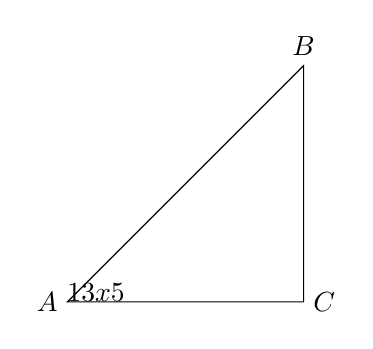
\begin{tikzpicture}
      \coordinate [label=left:$A$] (A) at (0,0);
      \coordinate [label=above:$B$] (B) at (3,3);
      \coordinate [label=right:$C$] (C) at (3,0);

      \draw (A) -- (B) -- (C) -- cycle;

     \tkzLabelSegment(A,B){$13$};
     \tkzLabelSegment[below=2pt](A,C){$x$};
     \tkzLabelSegment(B,C){$5$};
    \end{tikzpicture}

    \label{fig:find_tan_a}
  \end{figure}

  \solution

  \begin{align*}
    \textrm{\textbf{Step 1: }}&\textrm{According to the definition of $\tan(A)$} \\
    \tan(A) &= \frac{\textrm{opp}}{\textrm{adj}} = \frac{5}{x} \\
    \textrm{\textbf{Step 2: }}&\textrm{Find $x$ by using the Pythagorean Theorem $\tan(A)$} \\
    c^{2} &= a^{2} + b^{2} \\
    13^{2} &= 5^{2} + x^{2} \\
    169 &= 25 + x^{2} \\
    169 - 25 &= 25 - 25 + x^{2} \\
    144 &= x^{2} \\
    x &= \sqrt{144} = 12 \\
    \textrm{\textbf{Step 3: }}&\textrm{Substitute} \\
    \tan(A) &= \frac{\textrm{opp}}{\textrm{adj}} = \frac{5}{x} = \frac{5}{12} \approx 0.4167
  .\end{align*}

  \textbf{Solution:} $\tan(A) = \frac{5}{12} \approx  0.4167$
\end{exc}

% section the_tangent_ratio (end)

\section{Introducing the Sine and Cosine Ratios}
\label{sec:introducing_the_sine_and_cosine_ratios}

\begin{figure}[htpb]
  \centering

  \begin{tikzpicture}
    \coordinate [label=left:$A$] (A) at (0,0);
    \coordinate [label=above:$B$] (B) at (3,3);
    \coordinate [label=right:$C$] (C) at (3,0);

    \draw (A) -- (B) -- (C) -- cycle;

   \tkzLabelSegment(A,B){$c$};
   \tkzLabelSegment[below=2pt](A,C){$b$};
   \tkzLabelSegment(B,C){$a$};
  \end{tikzpicture}

  \label{fig:find_tan_a}
\end{figure}

In the right triangle $\triangle ABC$, $\sin(A) = \frac{a}{c}$. This value
depends only on the measure of the angle, and not on the lengths of the sides
of the particular triangle used.

In the right triangle, $\triangle ABC$, $\cos(A) = \frac{b}{c}$. This value
depends only on the measure of the angle, and not on the lengths of the sides
of the particular triangle used.

\begin{definition}[Sine]
  \label{def:sine}

  The \textbf{sine} (sin) of an acute angle of a right triangle is the ratio of
  the length of the leg opposite the acute angle to the length of the
  hypotenuse.

  \[ \sin(\theta) = \frac{\textrm{length of opposite side}}{\textrm{length of hypotenuse}}
                  = \frac{\textrm{opp}}{\textrm{hyp}} . \]
\end{definition}

\begin{definition}[Cosine]
  \label{def:cosine}

  The \textbf{cosine} (cos) of an acute angle of a right triangle is the ratio
  of the length of the leg adjacent the acute angle to the length of the
  hypotenuse.

  \[ \cos(\theta) = \frac{\textrm{length of adjacent side}}{\textrm{length of hypotenuse}}
                  = \frac{\textrm{adj}}{\textrm{hyp}} . \]
\end{definition}

As with tangent, the sine and cosine ratios are functions of an angle. The
values of $\sin(\theta)$ and $\cos(\theta)$ do not depend on the particular
triangle that contains this angle; they depend only on the value for $\theta$.

\subsection{Co-function Identity Between the Sine and Cosine}
\label{sub_sec:co_function_identity_between_the_sine_and_cosine}

In the following figure, $\cos(A) = \frac{5}{9}$ and $\sin(A) = \frac{5}{9}$.
If $\angle A$ and $\angle B$ are acute angles of the same right triangle, then

\begin{figure}[htpb]
  \centering

  \begin{tikzpicture}
    \coordinate [label=left:$A$] (A) at (0,0);
    \coordinate [label=above:$B$] (B) at (3,3);
    \coordinate [label=right:$C$] (C) at (3,0);

    \draw (A) -- (B) -- (C) -- cycle;

   \tkzLabelSegment(A,B){$9$};
   \tkzLabelSegment[below=2pt](A,C){$5$};
  \end{tikzpicture}

  \label{fig:find_tan_a}
\end{figure}

\[ \sin(A) = \cos(B) \textrm{ and } \cos(A) = \sin(B) . \]

It doesn't matter what the lengths of the sides are.

The sum of two acute angles in any right triangle is always $90^{\circ}$, so
you can express this fact with the following mathematical statement: $A^{\circ}
+ B^{\circ} = 90^{\circ}$, which leads to the following conclusions.

\begin{align*}
  A^{\circ} + B^{\circ} &= 90^{\circ} \\
  B^{\circ} &= 90^{\circ} - A^{\circ} \\
  \textrm{Now, you can rewrite }&\textrm{the equalities found previously} \\
  \sin(A) = \cos(B) &= \cos(90^{\circ} - A^{\circ}) \\
  \cos(A) = \sin(B) &= \sin(90^{\circ} - A^{\circ})
.\end{align*}

These equations are called \textit{co-function identities}.

\begin{identity}[Co-Function]
  \label{idn:co_function}

  \textbf{Co-function identities} for sine and cosine can be written as:

  \begin{align*}
    \sin(\theta) = \cos\left(\frac{\pi}{2} - \theta\right) \\
    \cos(\theta) = \sin\left(\frac{\pi}{2} - \theta\right)
  .\end{align*}
\end{identity}

% subsection co_function_identity_between_the_sine_and_cosine (end)

\subsection{Pythagorean Identity with Sine and Cosine}
\label{sub_sec:pythagorean_identity_with_sine_and_cosine}

\begin{align*}
  \textrm{\textbf{Step 1: }}&\textrm{According to the Pythagorean Theorem, you write:} \\
   &a^{2} + b^{2} = c^{2} \\
   &\frac{a^{2} + b^{2}}{c^{2}} = 1 \\
  \textrm{\textbf{Step 2: }}&\textrm{According to the definition of sine and cosine:} \\
   &\sin^{2}(A) = \frac{a}{c}, \textrm{ then } \sin^{2}(A) = \left(\frac{a}{c}\right)^{2} \\
   &\cos^{2}(A) = \frac{b}{c}, \textrm{ then } \cos^{2}(A) = \left(\frac{b}{c}\right)^{2} \\
  \textrm{\textbf{Step 3: }}&\textrm{Add the squares of the sine and the cosine:} \\
   &\sin^{2}(A) + \cos^{2}(A) = \left(\frac{a}{c}\right)^{2} + \left(\frac{b}{c}\right)^{2} = \frac{a^{2}}{c^{2}} + \frac{b^{2}}{c^{2}} = \frac{a^{2} + b^{2}}{c^{2}} \\
  \textrm{\textbf{Step 4: }}&\textrm{Because they are equal, you can write:} \\
   &\sin^{2}(A) + \cos^{2}(A) = \frac{a^{2} + b^{2}}{c^{2}} = 1
.\end{align*}

This expression is called the \textit{Pythagorean Identity}.

\begin{definition}[Pythagorean Identity]
  \label{def:pythagorean_identity}

  The \textbf{pythagorean identity} for the sine and cosine can be written as:

  \[ \sin^{2}(\theta) + \cos^{2}(\theta) = 1 . \]
\end{definition}

% subsection pythagorean_identity_with_sine_and_cosine (end)

\subsection{Values of Trig Functions for $0^{\circ}$ and $90^{\circ}$ Angles}
\label{sub_sec:values_of_trig_functions_for_0_circ_and_90_circ_angles}

We've been working with sine and cosine with only acute angles. But can we
define sine and cosine for $\sin(90^{\circ})$ or $\cos(0^{\circ})$ for example?

It's hard to explain the value of the trig functions for $0^{\circ}$ and
$90^{\circ}$ using triangles to explain it because using triangles is limiting.
But, for now, here's the proof.

\begin{proof}
  \label{prf:sin_90_equals_1}

  Make a triangle with two $90^{\circ}$ angles and $1$ $0^{\circ}$ angle.
  It would look something like this
  \begin{figure}[H]
    \centering

    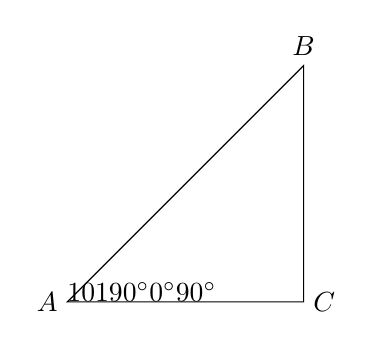
\begin{tikzpicture}
      \coordinate [label=left:$A$] (A) at (0,0);
      \coordinate [label=above:$B$] (B) at (3,3);
      \coordinate [label=right:$C$] (C) at (3,0);

      \draw (A) -- (B) -- (C) -- cycle;

      \tkzLabelSegment(A,B){$1$};
      \tkzLabelSegment(B,C){$0$};
      \tkzLabelSegment[below=2pt](A,C){$1$};

      \tkzMarkAngle[size=0.5cm](A,B,C)
      \tkzMarkAngle[size=0.5cm](C,A,B)
      \tkzMarkAngle[size=0.5cm](B,C,A)

      \tkzLabelAngle(A,B,C){$90^{\circ}$};
      \tkzLabelAngle(C,A,B){$0^{\circ}$};
      \tkzLabelAngle(B,C,A){$90^{\circ}$};
    \end{tikzpicture}

    \label{fig:sin_90_equals_1}
  \end{figure}

  Using the definitions of sine and cosine, we get the following
  \begin{align*}
    \sin(0^{\circ}) &= \frac{0}{1} = 0 \\
    \cos(0^{\circ}) &= \frac{1}{1} = 1 \\
    \sin(90^{\circ}) &= \frac{1}{1} = 1 \\
    \cos(90^{\circ}) &= \frac{0}{1} = 0
  .\end{align*}
\end{proof}

% subsection values_of_trig_functions_for_0_circ_and_90_circ_angles (end)

% section introducing_the_sine_and_cosine_ratios (end)

% chapter trig_functions_and_right_triangles (end)

\newpage
